% !TEX encoding = UTF-8 Unicode
\documentclass[12pt, a4paper]{article}




%Layout setup
% !TeX root = ./main.tex


%行高
\renewcommand{\baselinestretch}{1.5} 

%版型
\usepackage[a4paper,left=3cm,right=2cm,top=2.5cm,bottom=2.5cm]{geometry}

%數學
\usepackage{amsmath}

%表格
\usepackage{tabularx}
\usepackage{ltablex}

%中文設定
\usepackage{xeCJK} %讓中英文字體分開設置
% Noto Font: Download here: https://www.google.com/get/noto/#sans-hant
\setCJKmainfont{Noto Sans CJK TC}

\usepackage{booktabs} % 畫分隔線

%隱藏標題碼
\makeatletter
\renewcommand\@seccntformat[1]{}
\makeatother

%顏色
\usepackage[dvipsnames]{xcolor}

%標頭文字
\usepackage{fancyhdr} 


%超連結
\usepackage[unicode]{hyperref} %用 unicode防止中文亂碼
\usepackage{url}

\hypersetup{
    colorlinks=true,
    linkcolor=NavyBlue,
    filecolor=NavyBlue,      
    urlcolor=NavyBlue,
    citecolor=NavyBlue
} %超連結顏色

%文包圖
\usepackage{wrapfig}
\usepackage{subcaption}
\usepackage{stfloats} %caption footnote
%彩色方塊文字
\usepackage{tcolorbox}

%圖的文字
\usepackage[labelfont=bf, font={small}]{caption}

%中文package
\usepackage{CJKutf8}

%畫圖
\usepackage{tikz}
\usetikzlibrary{positioning}

%Reference
\usepackage[numbers]{natbib}
\bibliographystyle{unsrtnat}

\usepackage{multicol}


%Top row topics
\rhead{主題(右邊)}
\lhead{主題(左邊)}



%\date{} %Uncomment to hide date
\title{\textbf{主題}}

\author{邱紹庭%
\thanks{ 
    Correspondence: \href{mailto:r07945001@ntu.edu.tw}{\faInbox~r07945001@ntu.edu.tw}}; 
}


\begin{document}

\maketitle

\section{段落一:中文測試}

測試引用 \cite{mobility2020}. 

\section{段落二: English Section}

English is a West Germanic language first spoken in early medieval England, which has eventually become the leading language of international discourse in the 21st century

\subsection{段落二之一: 圖片, tcolorbox, table}

左邊的圖為 \ref{fig:pred-cities}; 右邊則為 \ref{fig:pred-compare}

%Figure: 子圖
\begin{figure}[htb]
    \centering 
    
    \begin{subfigure}[b]{0.4\textwidth}
        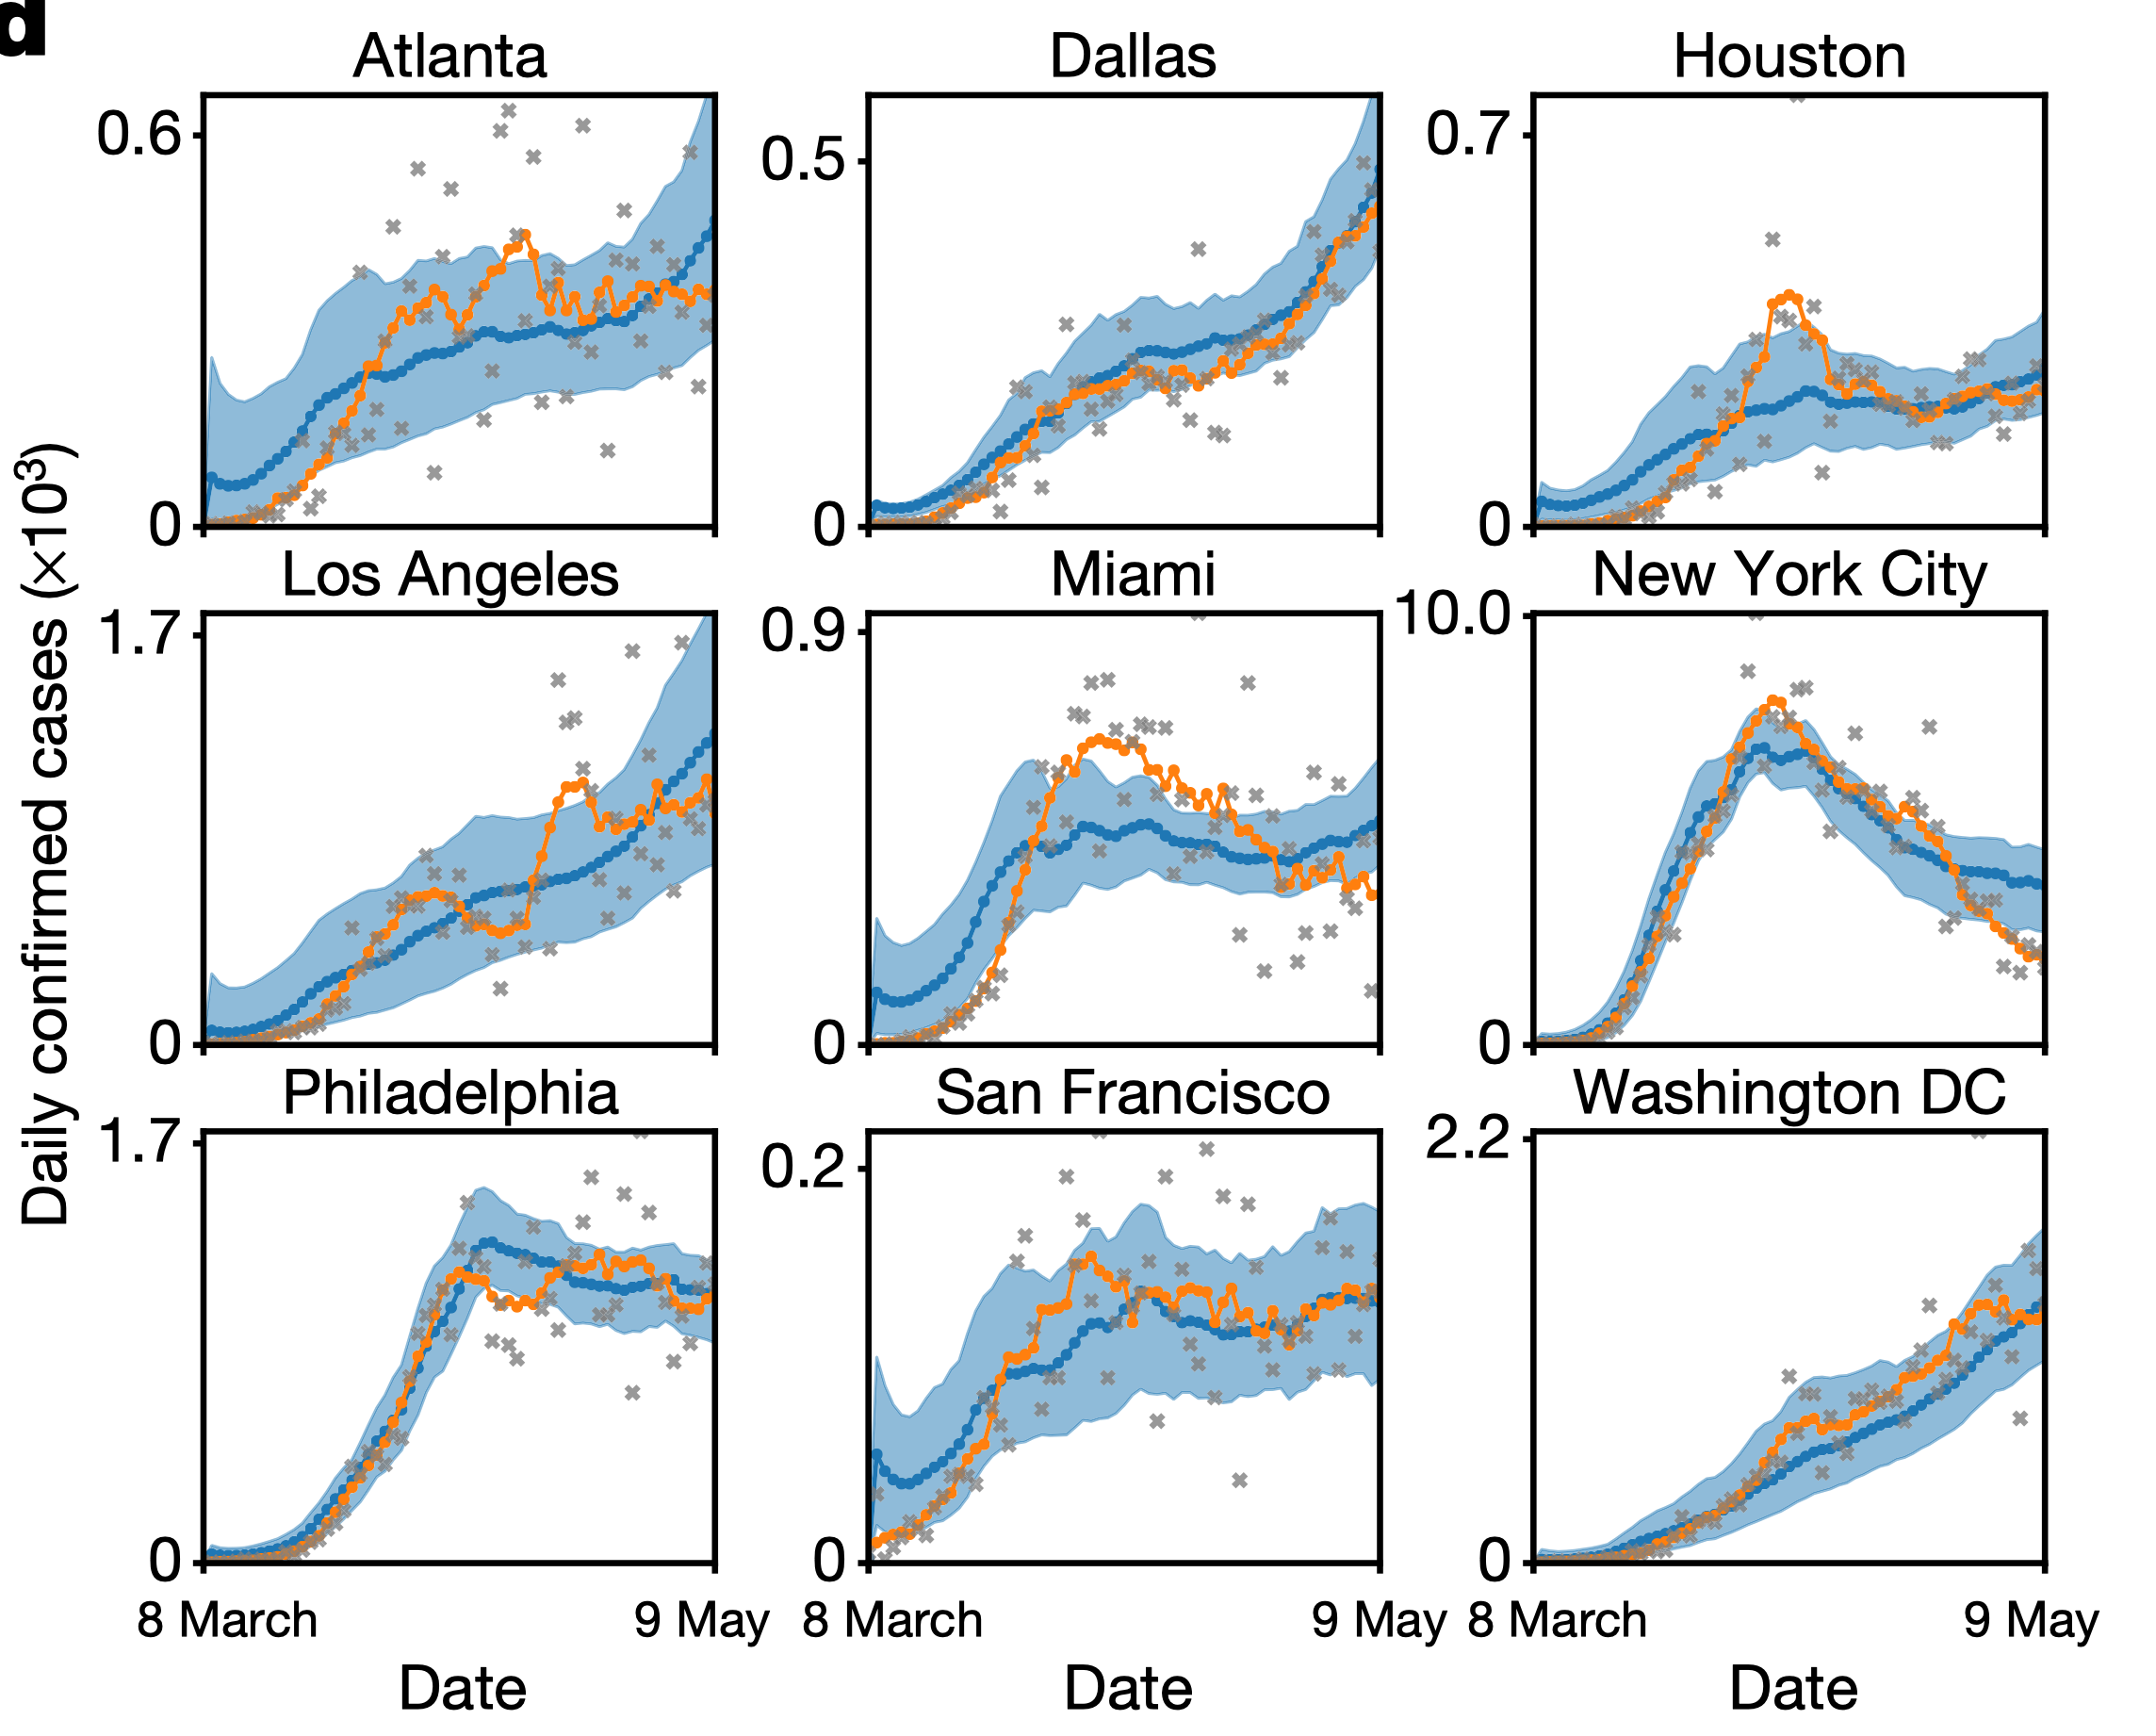
\includegraphics[width=\textwidth]{fig/sample.png}
         \caption{Sample 1}
         \label{fig:pred-cities}
    \end{subfigure} 
    \begin{subfigure}[b]{0.4\textwidth}
        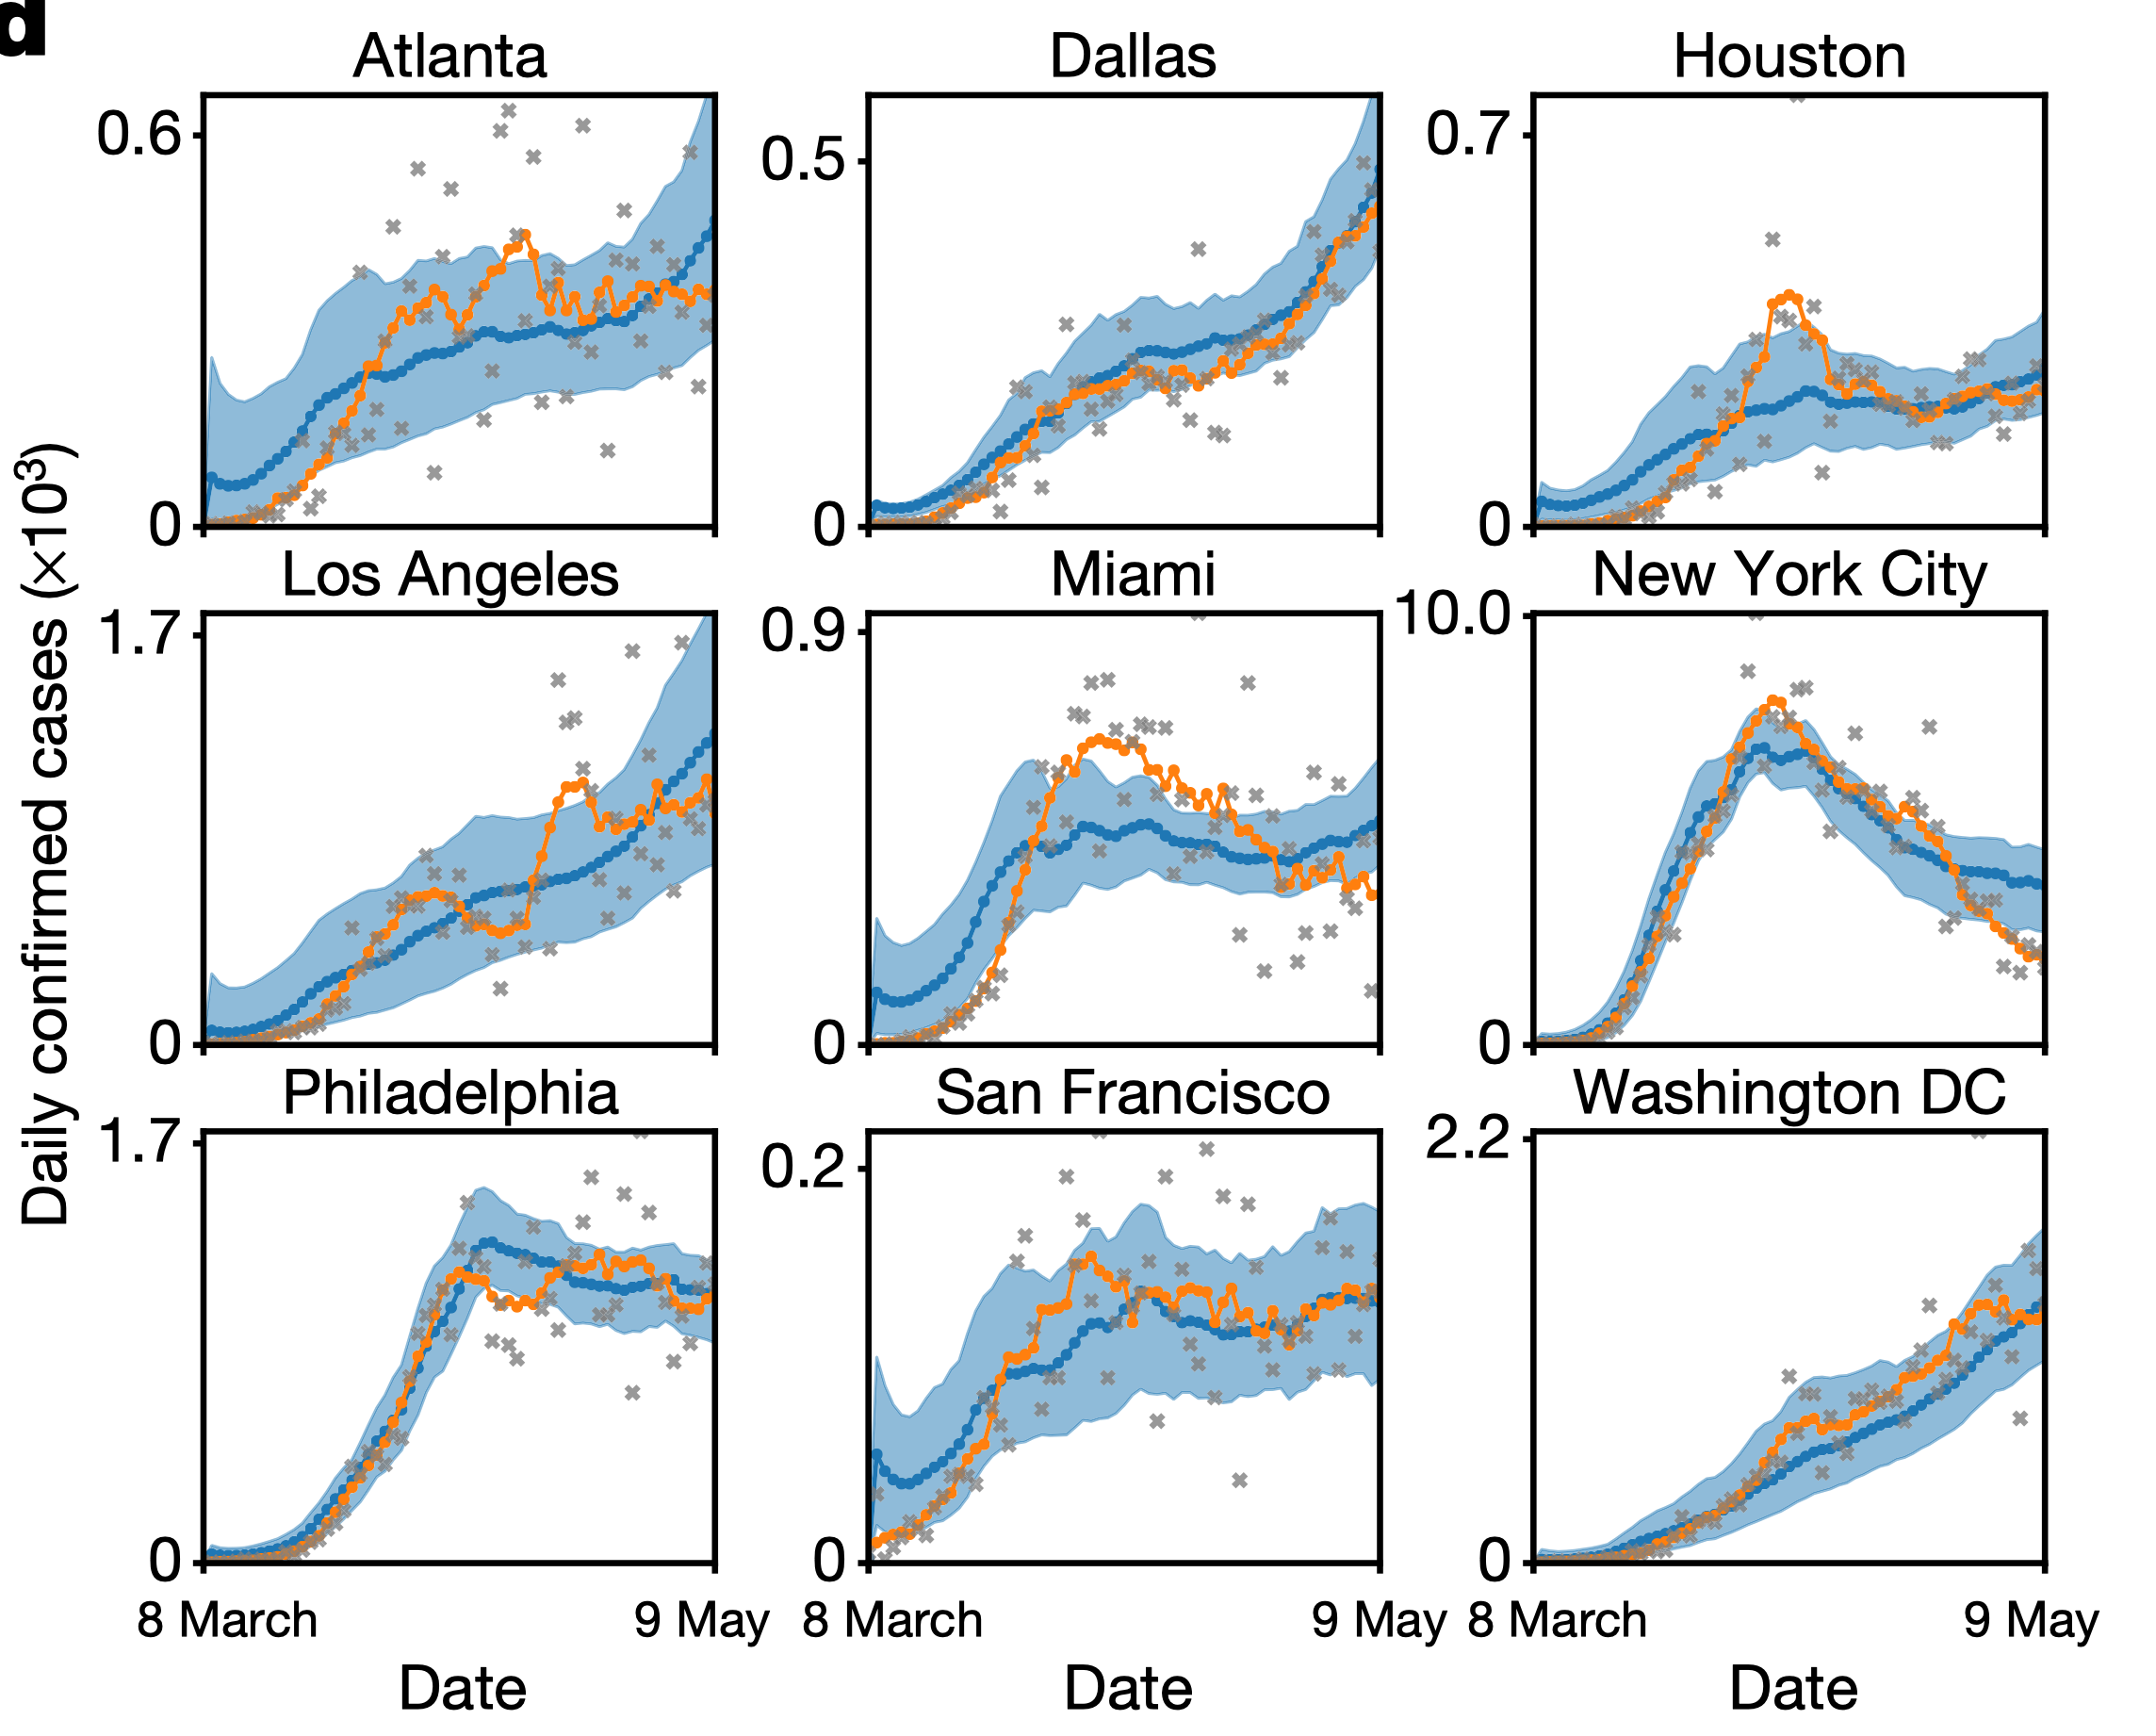
\includegraphics[width=\textwidth]{fig/sample.png}
        \caption{範例二}
        \label{fig:pred-compare}
    \end{subfigure}
    
    \caption{\citeauthor{mobility2020} 的 COVID-19 預測圖 \cite{mobility2020}) }
    \label{fig:pred}
\end{figure}

%色彩方塊
\begin{tcolorbox}[title=隨機 SEIR 模型]
    S從一個狀態轉換到下一個階段的人數以 $N$ 表示(狀態的分類在Fig.~\ref{fig:pred})。由於每個人轉換狀態的機率為 Bernoulli 機率分佈,群體下的機率則可以用下面的方程式表示:
    
    \begin{align} 
        N^{(t)}_{S_{c_i}\rightarrow E_{c_i}} & \sim  Binom(S^{(t)}_{c_1},  \lambda^{(t)}_{c_1}) \label{eq:N_S2E}\\
        N^{(t)}_{E_{c_i}\rightarrow 1_{c_i}} & \sim Binom(E^{(t)}_{c_i}, 1/\delta_{E}) \\
        N^{(t)}_{1_{c_1}\rightarrow R_{c_i}} & \sim Binom(I^{(t)}_{c_i}, 1/ \delta_{i})  
    \end{align}
    
    $N^{t}_{i\rightarrow j}$ 指的是在時間$t$時由$i$狀態轉換至$j$狀態的人數。
\end{tcolorbox}


%圖表
\begin{tabularx}{\linewidth}{ X  X   }
    \toprule
    
    \textbf{Data} & \textbf{連結}   \\ 

    \bottomrule
    
    A & \url{https://github.com/nytimes/covid-19-data}   \\ \hline
    A & \url{https://github.com/CSSEGISandData/COVID-19} \\ \hline
    \toprule
    \multicolumn{2}{l}{\textbf{預測工具}} \\ 
    \bottomrule
    SEIR 的 deterministic model (Python)\citep{mobility2020} & \url{https://github.com/ihmeuw/covid-model-seiir-pipeline/} \\ \hline
    \bottomrule
\end{tabularx}

% 輸出文獻
\bibliography{library}


\end{document}